\documentclass{article}

\usepackage[utf8]{inputenc}
\usepackage[T1]{fontenc}
\usepackage[portuguese]{babel}
\usepackage{amsmath}
\usepackage{bbm}
\usepackage{graphicx}
\usepackage{float}

\usepackage{pgf}
\usepackage{tikz}
\usepackage{circuitikz}
\usetikzlibrary{arrows,automata}

\graphicspath{ {./res/img/} }


\title{Circuitos Lógicos - Preparação 02}
\author{
    Rodrigo Seiji Piubeli Hirao - 186837
}
\date{\today}

\begin{document}
    \maketitle
    \newpage
    \tableofcontents
    \newpage
    \listoffigures
    \newpage

    \section{Tipos de Flip-Flops}

        Flip Flops são Latch que funcionam apenas com borda de subida. Ou seja, Elas armazenam um dado e só podem ser atualizadas no momento que o clock mudar de 0 para 1.

        \subsection{JK}

            O flip flop JK facilita a utilização do sistema criando uma entrada (J) para ativar o valor armazenado e outra (K) para desativar, sendo que as duas juntas colocam o valor oposto do atual.

            \begin{figure} [H] 
                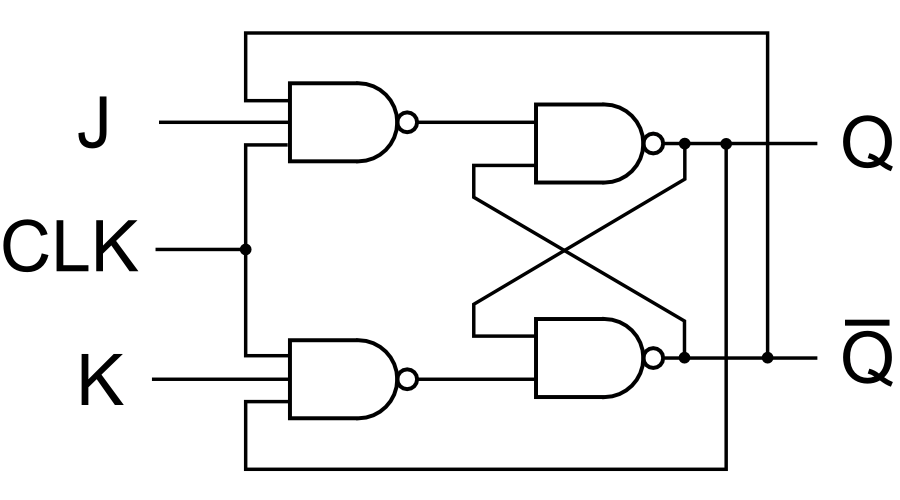
\includegraphics[width=8cm]{flipflop-jk.png}
                \caption{Flip-Flop JK}
                \label{fig:flipflop-jk}
            \end{figure}

            \paragraph{Fórmula}
            $Q = J\bar{Q} + \bar{K}Q$
            \newline
            \newline
            \begin{tabular}{||c c c c||}
                \hline
                CLK &   J   &   K   &   $Q_{próximo}$       \\
                \hline\hline
                0   &   -   &   -   &   $Q_{anterior}$      \\
                1   &   0   &   0   &   $Q_{anterior}$      \\
                1   &   0   &   1   &   1                   \\
                1   &   1   &   0   &   0                   \\
                1   &   1   &   1   &   $\bar{Q}_{anterior}$\\
                \hline
            \end{tabular}

        \subsection{D}

            O flip flop D facilita ainda mais a utilização do sistema criando uma entrada (D) que define o valor que será armazenado.

            \begin{figure} [H] 
                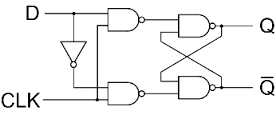
\includegraphics[width=8cm]{flipflop-d.png}
                \caption{Flip-Flop D}
                \label{fig:flipflop-d}
            \end{figure}

            \paragraph{Fórmula}
            $Q = D$
            \newline
            \newline
            \begin{tabular}{||c c c||}
                \hline
                CLK &   D   &   $Q_{próximo}$       \\
                \hline\hline
                0   &   -   &   $Q_{anterior}$      \\
                1   &   0   &   0                   \\
                1   &   1   &   1                   \\
                \hline
            \end{tabular}

        \subsection{T}

            O flip flop T serve apenas para alternar o valor armazenado, sendo útil para contadores binários.

            \begin{figure} [H] 
                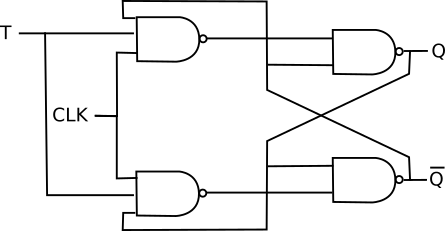
\includegraphics[width=8cm]{flipflop-t.png}
                \caption{Flip-Flop T}
                \label{fig:flipflop-t}
            \end{figure}

            \paragraph{Fórmula}
            $Q = T\bar{Q} + \bar{T}Q$
            \newline
            \newline
            \begin{tabular}{||c c c||}
                \hline
                CLK &   T   &   $Q_{próximo}$       \\
                \hline\hline
                0   &   -   &   $Q_{anterior}$      \\
                1   &   0   &   $Q_{anterior}$      \\
                1   &   1   &   $\bar{Q}_{anterior}$\\
                \hline
            \end{tabular}

    \section{Tipos de Máquinas de Estado}

        Uma Máquina de Estados é um circuito que permite a transição entre estados a partir de seu estado atual.

        \subsection{Máquina de Moore}
            A máquina de Moore é a máquina de estado no qual as entradas não afetam diretamente a saída.

            \begin{figure} [H] 
                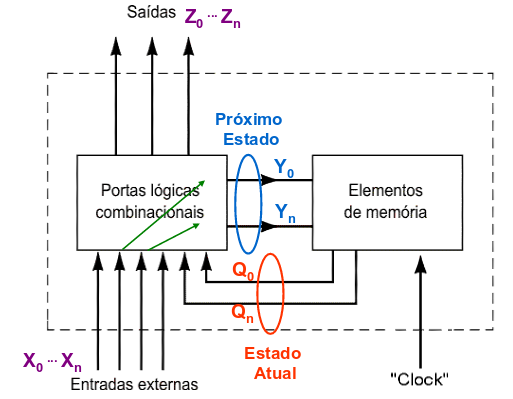
\includegraphics[width=8cm]{fsm-moore.png}
                \caption{Máquina de Moore}
                \label{fig:fsm-moore}
            \end{figure}

            Exemplo de um diagrama de estados
            \newline

            \begin{figure} [H] 
                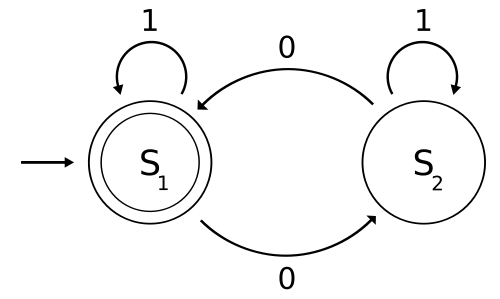
\includegraphics[width=8cm]{fsm-moore-diagram.png}
                \caption{Diagrama da Máquina de Moore}
                \label{fig:fsm-moore-diagram}
            \end{figure}

        \subsection{Máquina de Mealy}
            A máquina de Mealy é a máquina de estado no qual as entradas juntamente com o estado atual afetam diretamente a saída.

            \begin{figure} [H] 
                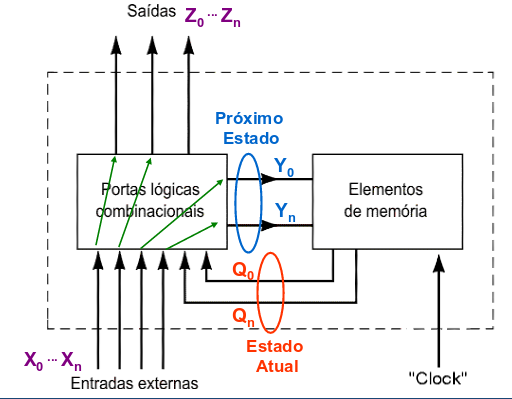
\includegraphics[width=8cm]{fsm-mealy.png}
                \caption{Máquina de Mealy}
                \label{fig:fsm-mealy}
            \end{figure}
            
            Exemplo de um diagrama de estados
            \newline

            \begin{figure} [H] 
                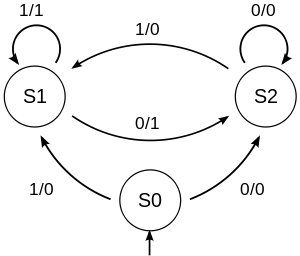
\includegraphics[width=8cm]{fsm-mealy-diagram.png}
                \caption{Diagrama da Máquina de Mealy}
                \label{fig:fsm-mealy-diagram}
            \end{figure}

    \section{Máquinas de Estado de 3 bits}

        Nesse circuito será usada uma máquina de estado de moore, pois este não depende da entrada.

        \subsection{Tabela Verdade}

            \begin{tabular}{||c c||}
                \hline
                Estado atual    &   Próximo Estado  \\
                \hline\hline
                000             &   001             \\
                001             &   010             \\
                010             &   011             \\
                011             &   100             \\
                100             &   101             \\
                101             &   110             \\
                110             &   111             \\
                111             &   000             \\
                \hline
            \end{tabular}

        \subsection{Diagrama de Estados}

            \begin{tikzpicture}[->,>=stealth',shorten >=1pt,auto,node distance=2.8cm, semithick]
                \tikzstyle{every state}=[fill=none,draw=black,text=black]

                \node[state]         (1)              {000};
                \node[state]         (2) [above of=1] {001};
                \node[state]         (3) [right of=2] {010};
                \node[state]         (4) [right of=3] {011};
                \node[state]         (5) [right of=4] {100};
                \node[state]         (6) [below of=5] {101};
                \node[state]         (7) [left  of=6] {110};
                \node[state]         (8) [left  of=7] {111};

                \path   (1) edge              node {X} (2)
                        (2) edge              node {X} (3)
                        (3) edge              node {X} (4)
                        (4) edge              node {X} (5)
                        (5) edge              node {X} (6)
                        (6) edge              node {X} (7)
                        (7) edge              node {X} (8)
                        (8) edge              node {X} (1);
            \end{tikzpicture}

        \subsection{Mapa de Karnaugh}

            \begin{tabular}{||c || c c c c||}
                \hline
                $D_2$   &   00  &   01  &   10  &   11  \\
                \hline\hline
                0       &   1   &   0   &   1   &   0   \\
                1       &   1   &   0   &   1   &   0   \\
                \hline
                \hline
                \hline
                $D_1$   &   00  &   01  &   10  &   11  \\
                \hline\hline
                0       &   0   &   1   &   1   &   0   \\
                1       &   0   &   1   &   1   &   0   \\
                \hline
                \hline
                \hline
                $D_0$   &   00  &   01  &   10  &   11  \\
                \hline\hline
                0       &   0   &   0   &   0   &   1   \\
                1       &   1   &   1   &   1   &   0   \\
                \hline
            \end{tabular}

        \subsection{Equações}

            Estado Atual -> $Q_0Q_1Q_2$
            \newline
            Próximo Estado -> $D_0D_1D_2$
            \newline

            Equações 
            \newline 
            \newline
            $D_2 = Q_2'$
            \newline
            $D_1 = (Q_1*Q_2')+(Q_1'*Q_2) = Q_1 \oplus Q_2$
            \newline
            $D_0 = (Q_0*Q_2)+(Q_0*Q_1')+(Q_0'*Q_1) = (Q_0*Q_2)+(Q_0 \oplus Q_1)$
    
        \subsection{Circuito}

            \begin{figure} [H] 
                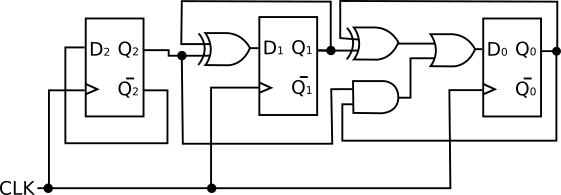
\includegraphics[width=8cm]{circuit-03.png}
                \caption{Máquina de Estado de 3 bits}
                \label{fig:circuit-03}
            \end{figure}

            Nota: para adicionar um reset, basta adicionar uma porta AND que tenha como entrada o botão de reset negado e a entrada representada acima em cada Flip Flop.
            \newline
            E o circuito pode ser simplificado da seguinte forma:

            \begin{figure} [H] 
                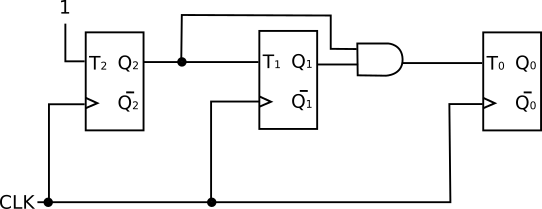
\includegraphics[width=8cm]{circuit-03-simple.png}
                \caption{Máquina de Estado de 3 bits (Simplificado)}
                \label{fig:circuit-03-simple}
            \end{figure}   

    \section{Contadores Síncronos}
        Contadores Síncronos são circuitos que, como o nome diz, 
        contam binariamente, aumentando seu contador a cada pulso do clock. 
        Estes podem contar até $2^n$, sendo n o número de flip flops presentes neste.
        \newline
        Mas para cascateá-los de forma a conseguirmos contar a um maior números precisamos usar um dos seguintes métodos:

        \subsection{Ripple Mode Carry Circuit}
            O primeiro modo é deixando eles em sequencia, 
            para que um só conte 1 número quando o anterior contar 16.
            \begin{figure} [H] 
                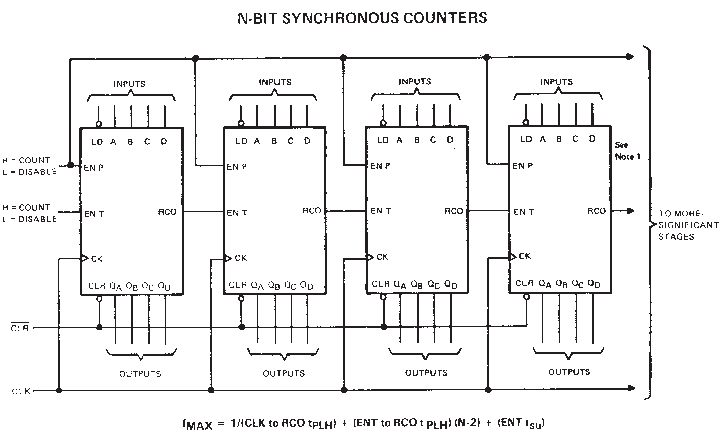
\includegraphics[width=8cm]{counter-cascading-01.png}
                \caption{Cascata de contadores - Ripple Mode Carry}
                \label{fig:counter-cascading-01}
            \end{figure}

        \subsection{Carry Look-Ahead Circuit}
            O segundo modo funciona do mesmo modo que o primeiro, 
            mas no primeiro caso o ENP do $3^o$ contador ficaria verdadeiro sempre, 
            enquanto no segundo modo ele só fica verdadeiro quando o $1^o$ contador acaba seu ciclo,
            caindo de 256 vezes, para 16.
            \begin{figure} [H] 
                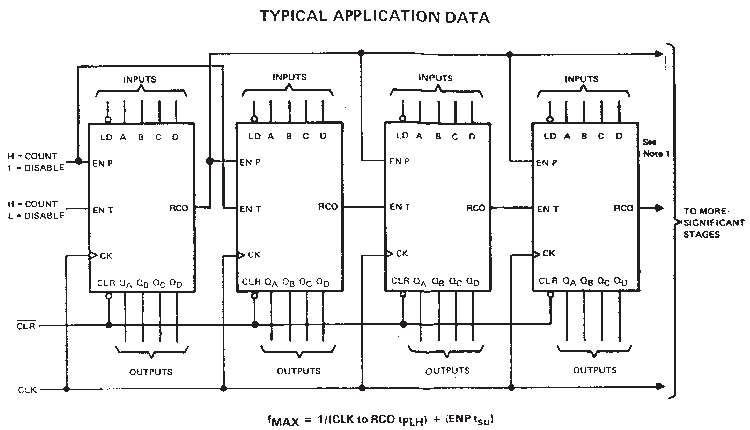
\includegraphics[width=8cm]{counter-cascading-02.png}
                \caption{Cascata de contadores - Carry Look-Ahead}
                \label{fig:counter-cascading-02}
            \end{figure}

\end{document}